\section*{Maven dependencies}
\label{sec:maven}
\definecolor{maroon}{rgb}{0.5,0,0}
\definecolor{darkgreen}{rgb}{0,0.5,0}
\lstdefinelanguage{XML}
{
	basicstyle=\ttfamily,
	morestring=[s]{"}{"},
	morecomment=[s]{?}{?},
	morecomment=[s]{!--}{--},
	commentstyle=\color{darkgreen},
	moredelim=[s][\color{black}]{>}{<},
	moredelim=[s][\color{red}]{\ }{=},
	stringstyle=\color{blue},
	identifierstyle=\color{maroon}
}

\begin{lstlisting}[language=XML, frame=htrbl, caption={Implementation of {\ttfamily pom.xml}}, label={lst:maven}, basicstyle=\footnotesize]
<?xml version="1.0" encoding="UTF-8"?>
<project xmlns="http://maven.apache.org/POM/4.0.0"
xmlns:xsi="http://www.w3.org/2001/XMLSchema-instance"
xsi:schemaLocation="http://maven.apache.org/POM/4.0.0
http://maven.apache.org/xsd/maven-4.0.0.xsd">
   <modelVersion>4.0.0</modelVersion>

   <groupId>com.runekrauss.e_compiler</groupId>
   <artifactId>e_compiler</artifactId>
   <version>0.0.1-SNAPSHOT</version>
   <build>
      <plugins>
         <plugin>
            <groupId>org.apache.maven.plugins</groupId>
            <artifactId>maven-assembly-plugin</artifactId>
            <executions>
               <execution>
                  <goals>
                     <goal>attached</goal>
                  </goals>
                  <phase>package</phase>
                  <configuration>
                     <descriptorRefs>
                        <descriptorRef>
                           jar-with-dependencies
                        </descriptorRef>
                     </descriptorRefs>
                     <archive>
                        <manifest>
                           <mainClass>
                              com.runekrauss.compiler.Main
                           </mainClass>
                        </manifest>
                     </archive>
                  </configuration>
               </execution>
            </executions>
         </plugin>
         <plugin>
            <groupId>org.apache.maven.plugins</groupId>
            <artifactId>maven-jar-plugin</artifactId>
            <version>3.0.2</version>
            <configuration>
               <archive>
                  <manifest>
                     <mainClass>com.runekrauss.compiler.Main</mainClass>
                     <addDefaultImplementationEntries>
                        true
                     </addDefaultImplementationEntries>
                     <addDefaultSpecificationEntries>
                        true
                     </addDefaultSpecificationEntries>
                     <addClasspath>true</addClasspath>
                  </manifest>
               </archive>
            </configuration>
         </plugin>
         <plugin>
            <groupId>org.apache.maven.plugins</groupId>
            <artifactId>maven-compiler-plugin</artifactId>
            <version>3.5.1</version>
            <configuration>
               <source>1.8</source>
               <target>1.8</target>
            </configuration>
         </plugin>
         <plugin>
            <groupId>com.coveo</groupId>
            <artifactId>fmt-maven-plugin</artifactId>
            <version>2.1.0</version>
            <configuration>
               <sourceDirectory>
                  src/main/java/com/runekrauss/compiler
               </sourceDirectory>
            </configuration>
            <executions>
               <execution>
                  <goals>
                     <goal>format</goal>
                  </goals>
               </execution>
            </executions>
         </plugin>
         <plugin>
            <groupId>org.apache.maven.plugins</groupId>
            <artifactId>maven-checkstyle-plugin</artifactId>
            <version>3.0.0</version>
            <configuration>
               <configLocation>google_checks.xml</configLocation>
            </configuration>
         </plugin>
      </plugins>
   </build>
   <dependencies>
      <dependency>
         <groupId>org.testng</groupId>
         <artifactId>testng</artifactId>
         <version>6.14.3</version>
         <scope>test</scope>
      </dependency>
      <dependency>
         <groupId>org.antlr</groupId>
         <artifactId>antlr4</artifactId>
         <version>4.7.1</version>
      </dependency>
      <dependency>
         <groupId>net.sourceforge</groupId>
         <artifactId>jasmin</artifactId>
         <version>2.4.0</version>
      </dependency>
   </dependencies>
</project>
\end{lstlisting}

\newpage

\section*{ASCII table}
\label{sec:ascii}
\begin{longtable}{|c|c|c|c||c|c|c|c|}
	\caption{Control characters and digits in ASCII}\\
	\hline
	Dec & Hex & Oct & Character & Dec & Hex & Oct & Character\\
	\hline
	0 & 0x00 & 000 & NUL & 32 & 0x20 & 040 & SP\\
	1 & 0x01 & 001 & SOH & 33 & 0x21 & 041 & ! \\
	2 & 0x02 & 002 & STX & 34 & 0x22 & 042 & "'\\
	3 & 0x03 & 003 & ETX & 35 & 0x23 & 043 & \# \\
	4 & 0x04 & 004 & EOT & 36 & 0x24 & 044 & \$ \\
	5 & 0x05 & 005 & ENQ & 37 & 0x25 & 045 & \% \\
	6 & 0x06 & 006 & ACK & 38 & 0x26 & 046 & \& \\
	7 & 0x07 & 007 & BEL & 39 & 0x27 & 047 & ' \\
	8 & 0x08 & 010 & BS & 40 & 0x28 & 050 & (  \\
	9 & 0x09 & 011 & TAB & 41 & 0x29 & 051 &  ) \\
	10 & 0x0A & 012 & LF & 42 & 0x2A & 052 & * \\
	11 & 0x0B & 013 & VT & 43 & 0x2B & 053 & + \\
	12 & 0x0C & 014 & FF & 44 & 0x2C & 054 & , \\
	13 & 0x0D & 015 & CR & 45 & 0x2D & 055 & - \\
	14 & 0x0E & 016 & SO & 46 & 0x2E & 056 & . \\
	15 & 0x0F & 017 & SI & 47 & 0x2F & 057 & / \\
	16 & 0x10 & 020 & DLE & 48 & 0x30 & 060 & 0 \\
	17 & 0x11 & 021 & DC1 & 49 & 0x31 & 061 & 1 \\
	18 & 0x12 & 022 & DC2 & 50 & 0x32 & 062 & 2 \\
	19 & 0x13 & 023 & DC3 & 51 & 0x33 & 063 & 3 \\
	20 & 0x14 & 024 & DC4 & 52 & 0x34 & 064 & 4 \\
	21 & 0x15 & 025 & NAK & 53 & 0x35 & 065 & 5 \\
	22 & 0x16 & 026 & SYN & 54 & 0x36 & 066 & 6 \\
	23 & 0x17 & 027 & ETB & 55 & 0x37 & 067 & 7 \\
	24 & 0x18 & 030 & CAN & 56 & 0x38 & 070 & 8 \\
	25 & 0x19 & 031 & EM & 57 & 0x39 & 071 & 9 \\
	26 & 0x1A & 032 & SUB & 58 & 0x3A & 072 & : \\
	27 & 0x1B & 033 & ESC & 59 & 0x3B & 073 & ; \\
	28 & 0x1C & 034 & FS & 60 & 0x3C & 074 & "< \\
	29 & 0x1D & 035 & GS & 61 & 0x3D & 075 & =\\
	30 & 0x1E & 036 & RS & 62 & 0x3E & 076 & "> \\
	31 & 0x1F & 037 & US & 63 & 0x3F & 077 & ? \\
	\hline
\end{longtable}
\newpage
\begin{longtable}{|c|c|c|c||c|c|c|c|}
	\caption{Letters in ASCII}\\
	\hline
	Dez & Hex & Okt & Zeichen & Dez & Hex & Okt & Zeichen\\
	\hline
	64 & 0x40 & 100 & @ & 96 & 0x60 & 140 & ` \\
	65 & 0x41 & 101 & A & 97 & 0x61 & 141 & a \\
	66 & 0x42 & 102 & B & 98 & 0x62 & 142 & b \\
	67 & 0x43 & 103 & C & 99 & 0x63 & 143 & c \\
	68 & 0x44 & 104 & D & 100 & 0x64 & 144 & d \\
	69 & 0x45 & 105 & E & 101 & 0x65 & 145 & e \\
	70 & 0x46 & 106 & F & 102 & 0x66 & 146 & f \\
	71 & 0x47 & 107 & G & 103 & 0x67 & 147 & g \\
	72 & 0x48 & 110 & H & 104 & 0x68 & 150 & h \\
	73 & 0x49 & 111 & I & 105 & 0x69 & 151 & i \\
	74 & 0x4A & 112 & J & 106 & 0x6A & 152 & j \\
	75 & 0x4B & 113 & K & 107 & 0x6B & 153 & k \\
	76 & 0x4C & 114 & L & 108 & 0x6C & 154 & l \\
	77 & 0x4D & 115 & M & 109 & 0x6D & 155 & m \\
	78 & 0x4E & 116 & N & 110 & 0x6E & 156 & n \\
	79 & 0x4F & 117 & O & 111 & 0x6F & 157 & o \\
	80 & 0x50 & 120 & P & 112 & 0x70 & 160 & p \\
	81 & 0x51 & 121 & Q & 113 & 0x71 & 161 & q \\
	82 & 0x52 & 122 & R & 114 & 0x72 & 162 & r \\
	83 & 0x53 & 123 & S & 115 & 0x73 & 163 & s \\
	84 & 0x54 & 124 & T & 116 & 0x74 & 164 & t \\
	85 & 0x55 & 125 & U & 117 & 0x75 & 165 & u \\
	86 & 0x56 & 126 & V & 118 & 0x76 & 166 & v \\
	87 & 0x57 & 127 & W & 119 & 0x77 & 167 & w \\
	88 & 0x58 & 130 & X & 120 & 0x78 & 170 & x \\
	89 & 0x59 & 131 & Y & 121 & 0x79 & 171 & y \\
	90 & 0x5A & 132 & Z & 122 & 0x7A & 172 & z \\
	91 & 0x5B & 133 & [ & 123 & 0x7B & 173 & \{ \\
	92 & 0x5C & 134 & $\backslash$ & 124 & 0x7C & 174 & $\mid$\\
	93 & 0x5D & 135 & ] & 125 & 0x7D & 175 & \} \\
	94 & 0x5E & 136 & \^{} & 126 & 0x7E & 176 & "~ \\
	95 & 0x5F & 137 & \_ & 127 & 0x7F & 177 & DEL \\
	\hline
\end{longtable}

\newpage

\section*{Rules for graph transformation of lexical analysis}
\label{sec:rules_graph_transformation}
\begin{figure}[bth]
	\centering
	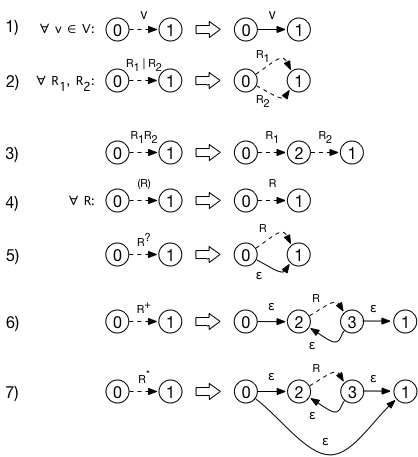
\includegraphics[scale=0.6]{./appendix/img/equivalence_automata_regex}
	\caption[Rules for graph transformation of lexical analysis]{Rules for graph transformation of lexical analysis}
	\label{fig:rules_graph_transformation}
\end{figure}
\noindent

\newpage

\section*{Generation of the lexer}
\label{sec:lexer}

\begin{lstlisting}[frame=htrbl, caption={Generation of {\ttfamily ELexer.java}}, label={lst:lexer}, basicstyle=\footnotesize]
public class ELexer extends Lexer {
   static { RuntimeMetaData.checkVersion("4.7.2", RuntimeMetaData
      .VERSION); }

   protected static final DFA[] _decisionToDFA;
   protected static final PredictionContextCache _sharedContextCache =
      new PredictionContextCache();
   public static final int
      T__0=1, T__1=2, T__2=3, T__3=4, T__4=5, T__5=6, T__6=7, T__7=8,
      ...  
      ASSIGN=51, QMARK=52, OPAREN=53, CPAREN=54, OBRACE=55, CBRACE=56, 
      OBRACKET=57, CBRACKET=58, OCBRACKET=59;
   public static String[] channelNames = {
      "DEFAULT_TOKEN_CHANNEL", "HIDDEN"
   };

   public static String[] modeNames = {
      "DEFAULT_MODE"
   };

   private static String[] makeRuleNames() {
      return new String[] {
         "T__0", "T__1", "T__2", "T__3", "T__4", "T__5", "T__6", "T__7",
         ... 
         "CBRACE", "OBRACKET", "CBRACKET", "OCBRACKET", "LETTER", "DIGIT"
      };
   }
   public static final String[] ruleNames = makeRuleNames();

   private static String[] makeLiteralNames() {
      return new String[] {
         null, "'use'", "'#define'", "'noMain'", "'print'", "'println'", 
         ... 
         "'='", "'\"'", "'('", "')'", "'{'", "'}'", "'['", "']'", "'[]'"
      };
   }
   private static final String[] _LITERAL_NAMES = makeLiteralNames();
   private static String[] makeSymbolicNames() {
      return new String[] {
         "BUILTINFUNCTION", "BOOL", "INTEGER", "FLOAT", "STRING", 
         ...
         "ASSIGN", "QMARK", "OPAREN", "CPAREN", "OBRACE", "OCBRACKET"
      };
   }
   private static final String[] _SYMBOLIC_NAMES = makeSymbolicNames();
   public static final Vocabulary VOCABULARY = new VocabularyImpl
      (_LITERAL_NAMES, _SYMBOLIC_NAMES);

   public static final String[] tokenNames;
   static {
      tokenNames = new String[_SYMBOLIC_NAMES.length];
      for (int i = 0; i < tokenNames.length; i++) {
         tokenNames[i] = VOCABULARY.getLiteralName(i);
         if (tokenNames[i] == null) {
            tokenNames[i] = VOCABULARY.getSymbolicName(i);
         }

         if (tokenNames[i] == null) {
            tokenNames[i] = "<INVALID>";
         }
      }
   }
...
   public ELexer(CharStream input) {
      super(input);
      _interp = new LexerATNSimulator(this,_ATN,_decisionToDFA,
         _sharedContextCache);
   }

   public String getGrammarFileName() { return "E.g4"; }

   public String[] getRuleNames() { return ruleNames; }
...
   public static final ATN _ATN =
      new ATNDeserializer().deserialize(_serializedATN.toCharArray());
   static {
      _decisionToDFA = new DFA[_ATN.getNumberOfDecisions()];
      for (int i = 0; i < _ATN.getNumberOfDecisions(); i++) {
         _decisionToDFA[i] = new DFA(_ATN.getDecisionState(i), i);
      }
   }
}
\end{lstlisting}

\newpage

\section*{Deterministic context-free language classes}
\label{sec:det_cfg_classes}

\begin{table}[bth]
	\centering
	\begin{tabular}{p{1.3cm}p{5.25cm}|p{1.6cm}|p{5.25cm}|}
		\hline
		\multicolumn{2}{|c|}{\textbf{Recursive descent parser (top-down)}} & \multicolumn{2}{c|}{\textbf{Shift reduce parser (bottom-up)}} \\ \hline
		\multicolumn{1}{|l|}{$LL(k)$}             & Predicts the next production using $k$ tokens (taking the stack contents into account). The left context must therefore be noted.           & $LR(k)$                     & Detects syntax errors as soon as possible and can parse all deterministic context-free languages. $LR(1)$ is canonical but relatively large parser tables are created.                   \\ \hline
		\multicolumn{1}{|l|}{$SLL(k)$}            & Indicates a subset of LL(k) where the left context does not have to be kept.            & $SLR(k)$                    & Creates simple parser tables and is relatively easy to implement. However, not all deterministic grammars can be handled with it. It does not have to scan all lookahead reductions.                   \\ \hline
		&               & $LALR(k)$                   & The complexity lies between \emph{LR} and \emph{SLR}. It therefore has a similar number of states to \emph{SLR} but recognizes more languages. It tries to combine states if goto tables and lookaheads are compatible. Conflicts are recognized by rules.                   \\ \cline{3-4} 
		&               & $GLR(k)$                    & Detects ambiguous grammars through rules and can be combined with \emph{LALR}.                   \\ \cline{3-4} 
	\end{tabular}
\end{table}

\newpage

\section*{Generation of the parser}
\label{sec:parser}

\begin{lstlisting}[frame=htrbl, caption={Generation of {\ttfamily EParser.java}}, label={lst:parser}, basicstyle=\footnotesize]
public class EParser extends Parser {
   static { RuntimeMetaData.checkVersion("4.7.2", RuntimeMetaData
      .VERSION); }

   protected static final DFA[] _decisionToDFA;
   protected static final PredictionContextCache _sharedContextCache =
      new PredictionContextCache();
   public static final int T__0=1, T__1=2, T__2=3, T__3=4, T__4=5, 
      T__5=6, T__6=7, T__7=8, T__8=9, 
      ...
      RULE_block = 24, RULE_statements = 25, RULE_formalParameters = 26, 
      RULE_dataType = 27, RULE_primitive = 28;
   private static String[] makeRuleNames() {
      return new String[] {
         "program", "includes", "module", "command", "statement", 
         "print", ..., "formalParameters", "dataType", "primitive"
      };
   }
   public static final String[] ruleNames = makeRuleNames();
   
   private static String[] makeLiteralNames() {
      return new String[] {
         "'use'", "'#define'", "'noMain'", "'print'", 
         ...
         "'else'", "'while'", "'asm'", "'invoke'", "'new'"
      };
   }
   private static final String[] _LITERAL_NAMES = makeLiteralNames();
   public static final Vocabulary VOCABULARY = new VocabularyImpl(
      _LITERAL_NAMES, _SYMBOLIC_NAMES);
   
   public static final String[] tokenNames;
   static {
      tokenNames = new String[_SYMBOLIC_NAMES.length];
      for (int i = 0; i < tokenNames.length; i++) {
         tokenNames[i] = VOCABULARY.getLiteralName(i);
         if (tokenNames[i] == null) {
            tokenNames[i] = VOCABULARY.getSymbolicName(i);
         }
   
         if (tokenNames[i] == null) {
            tokenNames[i] = "<INVALID>";
         }
      }
   }   
...
   public static class ProgramContext extends ParserRuleContext {
      public IncludesContext includes;
      public List<IncludesContext> incls = 
         new ArrayList<IncludesContext>();
      public NoMainContext noMain;
      public List<NoMainContext> noMains = 
         new ArrayList<NoMainContext>();
      public TerminalNode EOF() { return getToken(EParser.EOF, 0); }
      public List<CommandContext> command() {
         return getRuleContexts(CommandContext.class);
      }
      public CommandContext command(int i) {
         return getRuleContext(CommandContext.class,i);
      }
      public List<IncludesContext> includes() {
         return getRuleContexts(IncludesContext.class);
      }
      public IncludesContext includes(int i) {
         return getRuleContext(IncludesContext.class,i);
      }
      public List<NoMainContext> noMain() {
         return getRuleContexts(NoMainContext.class);
      }
      public NoMainContext noMain(int i) {
         return getRuleContext(NoMainContext.class,i);
      }
      public ProgramContext(ParserRuleContext parent, 
         int invokingState) {
         super(parent, invokingState);
      }
      public int getRuleIndex() { return RULE_program; }
      @Override
      public <T> T accept(ParseTreeVisitor<? extends T> visitor) {
         if ( visitor instanceof EVisitor ) return ((EVisitor<? extends
            T>)visitor).visitProgram(this);
         else return visitor.visitChildren(this);
      }
   }
   
   public final ProgramContext program() throws RecognitionException {
      ProgramContext _localctx = new ProgramContext(_ctx, getState());
      enterRule(_localctx, 0, RULE_program);
      int _la;
      try {
         enterOuterAlt(_localctx, 1);
         {
         setState(61);
         _errHandler.sync(this);
         _la = _input.LA(1);
         while (_la==T__0) {
            {
            {
            setState(58);
            ((ProgramContext)_localctx).includes = includes();
            ((ProgramContext)_localctx).incls.add(
               ((ProgramContext)_localctx).includes);
            }
            }
            setState(63);
            _errHandler.sync(this);
            _la = _input.LA(1);
         }
         setState(67);
         _errHandler.sync(this);
         _la = _input.LA(1);
         while (_la==T__1) {
            {
            {
            setState(64);
            ((ProgramContext)_localctx).noMain = noMain();
            ((ProgramContext)_localctx).noMains.add(
               ((ProgramContext)_localctx).noMain);
            }
            }
            setState(69);
            _errHandler.sync(this);
            _la = _input.LA(1);
         }
         ...
      return _localctx;
   }  
...
   public final IncludesContext includes() throws RecognitionException 
      { ... }     
...
   public static final ATN _ATN =
      new ATNDeserializer().deserialize(_serializedATN.toCharArray());
   static {
      _decisionToDFA = new DFA[_ATN.getNumberOfDecisions()];
      for (int i = 0; i < _ATN.getNumberOfDecisions(); i++) {
         _decisionToDFA[i] = new DFA(_ATN.getDecisionState(i), i);
      }
   }
}    
\end{lstlisting}

\newpage

\section*{Implementation of the exceptions}
\label{sec:exceptions}

\begin{lstlisting}[frame=htrbl, caption={Implementation of {\ttfamily AlreadyDefinedVariableException.java}}, label={lst:already_defined_variable_exception}, basicstyle=\footnotesize]
public class AlreadyDefinedVariableException extends CompilerException {
   private String id;

   public AlreadyDefinedVariableException(Token var) {
      super(var);
      id = var.getText();
   }

   @Override
   public String getMessage() {
      return line + ":" + column + 
      " Already defined variable: <" + id + ">;";
   }
}
\end{lstlisting}

\begin{lstlisting}[frame=htrbl, caption={Implementation of {\ttfamily UndeclaredVariableException.java}}, label={lst:undeclared_variable_exception}, basicstyle=\footnotesize]
public class UndeclaredVariableException extends CompilerException {
   private String id;

   public UndeclaredVariableException(Token var) {
      super(var);
      id = var.getText();
   }

   @Override
   public String getMessage() {
      return line + ":" + column + 
      " Undeclared variable: <" + id + ">;";
   }
}
\end{lstlisting}

\begin{lstlisting}[frame=htrbl, caption={Implementation of {\ttfamily UndefinedFunctionException.java}}, label={lst:undefined_function_exception}, basicstyle=\footnotesize]
public class UndefinedFunctionException extends CompilerException {
   private String id;
   
   public UndefinedFunctionException(Token func) {
      super(func);
      id = func.getText();
   }

   @Override
   public String getMessage() {
      return line + ":" + column + " Undefined function: <" + id + ">;";
   }
}
\end{lstlisting}

\begin{lstlisting}[frame=htrbl, caption={Implementation of {\ttfamily AlreadyDefinedFunctionException.java}}, label={lst:already_defined_function_exception}, basicstyle=\footnotesize]
public class AlreadyDefinedFunctionException extends CompilerException {
   private String id;

   public AlreadyDefinedFunctionException(Token func) {
      super(func);
      id = func.getText();
   }

   @Override
   public String getMessage() {
      return line + ":" + column + " Already defined function: <"+id+">;";
   }
}
\end{lstlisting}

\begin{lstlisting}[frame=htrbl, caption={Implementation of {\ttfamily UndeclaredStructException.java}}, label={lst:undeclared_struct_exception}, basicstyle=\footnotesize]
public class UndeclaredStructException extends CompilerException {
   private final String id;

   public UndeclaredStructException(final Token var) {
      super(var);
      id = var.getText();
   }

   @Override
   public String getMessage() {
      return line + ":" + column + " Undeclared struct: <" + id + ">;";
   }
}
\end{lstlisting}

\begin{lstlisting}[frame=htrbl, caption={Implementation of {\ttfamily AlreadyDeclaredStructException.java}}, label={lst:already_declared_struct_exception}, basicstyle=\footnotesize]
public class AlreadyDeclaredStructException extends CompilerException {
   private final String id;

   public AlreadyDeclaredStructException(final Token var) {
      super(var);
      id = var.getText();
   }

   @Override
   public String getMessage() {
      return line + ":" + column + " Already declared struct: <" + id + 
         ">;";
   }
}
\end{lstlisting}

\begin{lstlisting}[frame=htrbl, caption={Implementation of {\ttfamily WrongDataTypeException.java}}, label={lst:wrong_data_type_exception}, basicstyle=\footnotesize]
public class WrongDataTypeException extends CompilerException {
   /** Tracks all of the nodes in the AST traversed by the parser. */
   private final String track;

   public WrongDataTypeException(final Token track) {
      super(track);
      this.track = track.getText();
   }

   @Override
   public String getMessage() {
      return line + ":" + column + " Wrong data type: <" + track + ">;";
   }
}
\end{lstlisting}

\begin{lstlisting}[frame=htrbl, caption={Implementation of {\ttfamily UnknownBuiltinFunctionException.java}}, label={lst:unknown_builtin_function_exception}, basicstyle=\footnotesize]
public class UnknownBuiltinFunctionException extends CompilerException {
   private final String id;
   public UnknownBuiltinFunctionException(final Token func) {
      super(func);
      id = func.getText();
   }
   @Override
   public String getMessage() {
      return line + ":" + column + " The built-in function could not be 
         found: <" + id + ">;";
   }
}
\end{lstlisting}

\begin{lstlisting}[frame=htrbl, caption={Implementation of {\ttfamily UnknownModuleException.java}}, label={lst:unknown_module_exception}, basicstyle=\footnotesize]
public class UnknownModuleException extends CompilerException {
   private final String id;
   public UnknownModuleException(final Token mod) {
      super(mod);
      id = mod.getText();
   }
   @Override
   public String getMessage() {
      return line + ":" + column + " The module could not be found: <" + 
         id + ">;";
   }
}
\end{lstlisting}

\newpage

\section*{Jasmin instructions}
\label{sec:jasmin_instructions}
\begin{table}[bth]
	\centering
	\caption{Relevant instructions of Jasmin}
	\label{tab:jasmin_instructions}
	\begin{tabular}{|l|l|p{10cm}|}
		\hline
		\multicolumn{1}{|c|}{\textbf{Instruction}} & \multicolumn{1}{|c|}{\textbf{Opcode}} & \multicolumn{1}{|c|}{\textbf{Description}} \\\hline
		\texttt{dup} & 0x59 & This pops the top single-word value off the operand stack and then pushes that value twice. \\\hline
		\texttt{f2i} & 0x8B & Pops a single precision float off of the stack, casts it to a 32-bit integer and pushes the integer value back onto the stack. \\\hline
		\texttt{getstatic} & 0xB2 & Pops a reference to an object from the stack, retrieves the value of the static field (also known as a class field) identified by a field specification from the reference and pushes the one-word or two-word value onto the operand stack. \\\hline
		\texttt{goto} & 0xA7 & Causes execution to branch to the instruction at the address (pc + branchoffset), where pc is the address of the goto opcode in the bytecode and branchoffset is a 16-bit signed integer parameter that immediately follows the goto opcode in the bytecode. \\\hline
		\texttt{iadd} & 0x60 & Pops two integers from the stack, adds them and pushes the integer result back onto the stack. \\\hline
		\texttt{idiv} & 0x6C & Pops the top two integers from the operand stack and divides the second-from top integer by the top integer. The quotient result is truncated to the nearest integer and placed on the stack. \\\hline
		\texttt{ifeq} & 0x99 & Pops the top integer off the operand stack. If the integer equals zero, execution branches to the address (pc + branchoffset).\\\hline
		\texttt{ifne} & 0x9A & Pops the top integer off the operand stack. If the integer does not equal zero, execution branches to the address (pc + branchoffset).\\\hline
		\texttt{if\_icmplt} & 0xA1 & Pops the top two ints off the stack and compares them.\\\hline
		\texttt{iload} & 0x15 & Loads a value from the table regarding variables at a desired position onto the stack. \\\hline
		\texttt{imul} & 0x68 & Pops the top two integers from the operand stack, multiplies them and pushes the result back onto the stack. \\\hline
		\texttt{invokespecial} & 0xB7 & Is used in certain special cases to invoke a method. \\\hline
		\texttt{invokestatic} & 0xB8 & Calls a static method (also known as a class method). \\\hline	
	\end{tabular}
\end{table}

\newpage

\begin{table}[bth]
	\centering
	\caption{Relevant instructions of Jasmin 2}
	\label{tab:jasmin_instructions2}
	\begin{tabular}{|l|l|p{10cm}|}
		\hline
		\multicolumn{1}{|c|}{\textbf{Instruction}} & \multicolumn{1}{|c|}{\textbf{Opcode}} & \multicolumn{1}{|c|}{\textbf{Description}} \\\hline
		\texttt{invokevirtual} & 0xB6 & Dispatches a Java method. It is used in Java to invoke all methods except interface methods. \\\hline
		\texttt{irem} & 0x70 & Pops two integers from the operand stack, divides value2 by value1, computes the remainder and pushes the integer remainder back onto the stack. \\\hline
		\texttt{ireturn} & 0xAC & Pops an integer from the top of the stack and pushes it onto the operand stack of the invoker. \\\hline
		\texttt{ishl} & 0x78 & Pops two integers off the stack. Shifts \emph{value2} left by the amount indicated in the five low bits of \emph{value1}. The integer result is then pushed back onto the stack. \\\hline
		\texttt{ishr} & 0x7A & Pops two integers off the stack. Shifts \emph{value1} right by the amount indicated in the five low bits of \emph{value2}. The integer result is then pushed back onto the stack. \emph{value1} is shifted arithmetically (preserving the sign extension). \\\hline	
		\texttt{istore} & 0x36 & Gets the topmost integer from the stack and places it in the table regarding the variables. \\\hline
		\texttt{isub} & 0x64 & Pops two integers from the stack, subtracts the top one from the second one and pushes the result back onto the stack. \\\hline
		\texttt{ixor} & 0x82 & Pops two integers off the operand stack. Computes the bitwise exclusive or of \emph{value1} and \emph{value2}. The integer result replaces \emph{value1} and \emph{value2} on the stack. \\\hline
		\texttt{i2f} & 0x86 & Pops an integer off the operand stack, casts it into a single-precision float and pushes the float back onto the stack.  \\\hline
		\texttt{ldc} & 0x12 & Loads a constant value onto the stack. \\\hline
		\texttt{new} & 0xBB & Determines the size in bytes of instances of the given class and allocates memory for the new instance from the garbage collected heap. \\\hline
		\texttt{newarray} & 0xBC & Pops a positive integer off the stack and constructs an array for holding \emph{n} elements of the given type. \\\hline
		\texttt{putstatic} & 0xB3 & Sets the value of the static field identified by a field specification to the single or double word value on the operand stack. \\\hline
	\end{tabular}
\end{table}

\textbf{Note}: The \emph{value2} is always below \emph{value1}. There are prefixes for several data types for different operators. For example, there is \texttt{fadd} for the addition of floating point numbers. There are also special Jasmin commands like \texttt{.field} to add an attribute to a class.

\newpage

\section*{Example of an E program}
\label{sec:eprogram}

\begin{lstlisting}[frame=htrbl, caption={Implementation of {\ttfamily main.e}}, label={lst:eprogram}, basicstyle=\footnotesize]
// Different library imports
use(e.std.math)

/**
 * A point in a two-dimensional space
 *
 * @author Rune Krauss
 */
struct Point1 {
   int x;
   int y;
}

/**
 * One more point in a two-dimensional space
 *
 * @author Rune Krauss
 */
struct Point2 {
   float x;
   float y;
}

/**
 * Finds the square root of an integer.
 *
 * @param x Integer
 * @return Square root
 */
int sqrt(int x) {
   int result;
   // Illegal
   if (x < 0) {
      result = -1;
   }
   // Base cases
   if (x == 0 || x == 1) {
      result = x;
   } else {
      int temp = 1;
      int i = 1;
      /*
       * Starting from 1, try all numbers until
       * i*i is greater than or equal to x
       */
      while (temp <= x) {
         i = i + 1;
         temp = i * i;
      }
      result = i - 1;
   }
   return result;
}

/**
 * Calculates the distance between two points.
 *
 * @param x1 X value of the first point
 * @param y1 Y value of the first point
 * @param x2 X value of the second point
 * @param y2 Y value of the second point
 * @return Distance
 */
int dist(int x1, int y1, int x2, int y2) {
   int part1 = math.square(x2-x1): int;
   int part2 = math.square(y2-y1): int;
   int result = sqrt(part1+part2);
   return result;
}

// Create different points
Point1 p1 = new Point1(5, 2);
Point2 p2 = new Point2(3.7, 4.1);
p1.x = 1;

// Calculate the distance between these points
int dist = dist(p1.x, p1.y, toInt(p2.x), toInt(p2.y));

// Save the result in a list
int[] list = new int[3];
list[0] = dist;

// Output some information about the list
String txt = "Result: ";
String output = append(txt, toString(dist));

print(output); // Result: 2
\end{lstlisting}

\newpage

\begin{figure}[h!]
	\centering
	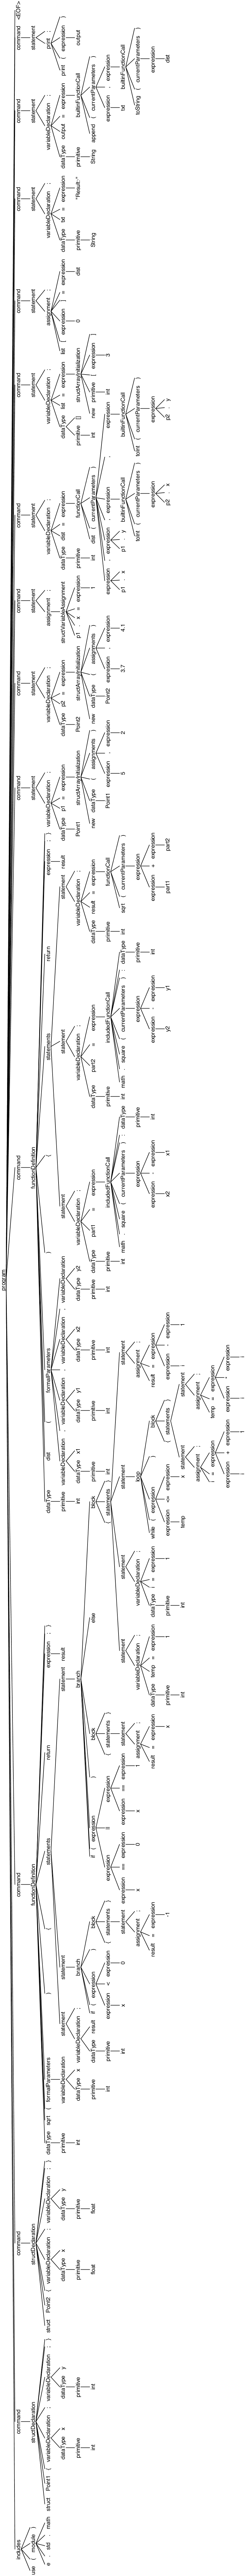
\includegraphics[scale=0.07]{./img/parse_tree}
	\caption[AST of {\ttfamily main.e}]{AST of {\ttfamily main.e}}
	\label{fig:parse_tree}
\end{figure}
\noindent

\newpage

\begin{lstlisting}[frame=htrbl, caption={Generated code of {\ttfamily main.e}}, label={lst:codeMain}, basicstyle=\footnotesize]
.class public e_test_main
.super java/lang/Object

.field public static v0 Lstruct_e_test_main0;
.field public static v1 Lstruct_e_test_main1;
.field public static v2 I
.field public static v3 [I
.field public static v4 Ljava/lang/String;
.field public static v5 Ljava/lang/String;

.method public static sqrt(I)I
.limit locals 4
.limit stack 4

iload 0
ldc 0
if_icmplt onCmpTrue1
ldc 0
goto endCmp1
onCmpTrue1:
ldc 1
endCmp1:
ifne onTrue1

goto endIf1
onTrue1:
ldc -1
istore 1

endIf1:

iload 0
ldc 0
if_icmpeq onCmpTrue2
ldc 0
goto endCmp2
onCmpTrue2:
ldc 1
endCmp2:
ifne onOrTrue1
iload 0
ldc 1
if_icmpeq onCmpTrue3
ldc 0
goto endCmp3
onCmpTrue3:
ldc 1
endCmp3:
ifne onOrTrue1
ldc 0
goto endOr1
onOrTrue1:
ldc 1
endOr1:

ifne onTrue2
ldc 1
istore 2
ldc 1
istore 3
beginLoop1:
iload 2
iload 0
if_icmple onCmpTrue4
ldc 0
goto endCmp4
onCmpTrue4:
ldc 1
endCmp4:
ifeq endLoop1
iload 3
ldc 1
iadd
istore 3

iload 3
iload 3
imul
istore 2

goto beginLoop1
endLoop1:

iload 3
ldc 1
isub
istore 1

goto endIf2
onTrue2:
iload 0
istore 1

endIf2:

iload 1
ireturn
.end method

.method public static dist(IIII)I
.limit locals 7
.limit stack 5
iload 2
iload 0
isub

invokestatic e_std_math/square(I)I
istore 4
iload 3
iload 1
isub

invokestatic e_std_math/square(I)I
istore 5
iload 4
iload 5
iadd

invokestatic e_test_main/sqrt(I)I
istore 6
iload 6
ireturn
.end method


.method public static main([Ljava/lang/String;)V
.limit stack 9
.limit locals 1

new struct_e_test_main0
dup
invokespecial struct_e_test_main0/<init>()V
putstatic e_test_main/v0 Lstruct_e_test_main0;
getstatic e_test_main/v0 Lstruct_e_test_main0;
ldc 5
putfield struct_e_test_main0/a0 I
getstatic e_test_main/v0 Lstruct_e_test_main0;
ldc 2
putfield struct_e_test_main0/a1 I
getstatic e_test_main/v0 Lstruct_e_test_main0;

putstatic e_test_main/v0 Lstruct_e_test_main0;
new struct_e_test_main1
dup
invokespecial struct_e_test_main1/<init>()V
putstatic e_test_main/v1 Lstruct_e_test_main1;
getstatic e_test_main/v1 Lstruct_e_test_main1;
ldc 3.7
putfield struct_e_test_main1/a0 F
getstatic e_test_main/v1 Lstruct_e_test_main1;
ldc 4.1
putfield struct_e_test_main1/a1 F
getstatic e_test_main/v1 Lstruct_e_test_main1;

putstatic e_test_main/v1 Lstruct_e_test_main1;
getstatic e_test_main/v0 Lstruct_e_test_main0;
ldc 1
putfield struct_e_test_main0/a0 I

getstatic e_test_main/v0 Lstruct_e_test_main0;
getfield struct_e_test_main0/a0 I

getstatic e_test_main/v0 Lstruct_e_test_main0;
getfield struct_e_test_main0/a1 I

getstatic e_test_main/v1 Lstruct_e_test_main1;
getfield struct_e_test_main1/a0 F

f2i
getstatic e_test_main/v1 Lstruct_e_test_main1;
getfield struct_e_test_main1/a1 F

f2i

invokestatic e_test_main/dist(IIII)I
putstatic e_test_main/v2 I
ldc 3
newarray int

putstatic e_test_main/v3 [I
getstatic e_test_main/v3 [I
ldc 0
getstatic e_test_main/v2 I
iastore

ldc "Result: "
putstatic e_test_main/v4 Ljava/lang/String;
new java/lang/StringBuffer
dup
invokespecial java/lang/StringBuffer/<init>()V
getstatic e_test_main/v4 Ljava/lang/String;

invokevirtual java/lang/StringBuffer/append(Ljava/lang/String;)Ljava/
   lang/StringBuffer;
getstatic e_test_main/v2 I
invokestatic java/lang/Integer.toString(I)Ljava/lang/String;

invokevirtual java/lang/StringBuffer/append(Ljava/lang/String;)Ljava/
   lang/StringBuffer;
invokevirtual java/lang/StringBuffer/toString()Ljava/lang/String;
putstatic e_test_main/v5 Ljava/lang/String;
getstatic java/lang/System/out Ljava/io/PrintStream;
getstatic e_test_main/v5 Ljava/lang/String;
invokevirtual java/io/PrintStream/print(Ljava/lang/String;)V


return

.end method
\end{lstlisting}

\begin{lstlisting}[frame=htrbl, caption={Generated code of struct {\ttfamily Point1}}, label={lst:codePoint1}, basicstyle=\footnotesize]
.class struct_e_test_main0
.super java/lang/Object

.field public a0 I
.field public a1 I
.method public <init>()V
aload_0
invokespecial java/lang/Object/<init>()V
return
.end method
\end{lstlisting}

\begin{lstlisting}[frame=htrbl, caption={Generated code of struct {\ttfamily Point2}}, label={lst:codePoint2}, basicstyle=\footnotesize]
.class struct_e_test_main1
.super java/lang/Object

.field public a0 F
.field public a1 F
.method public <init>()V
aload_0
invokespecial java/lang/Object/<init>()V
return
.end method
\end{lstlisting}

\begin{lstlisting}[frame=htrbl, caption={Generated code of {\ttfamily math.e}}, label={lst:codeMath}, basicstyle=\footnotesize]
.class public e_std_math
.super java/lang/Object



.method public static square(I)I
.limit locals 1
.limit stack 2
iload 0
iload 0
imul
ireturn
.end method

.method public static max(II)I
.limit locals 3
.limit stack 3
iload 0
istore 2
iload 1
iload 0
if_icmpgt onCmpTrue1
ldc 0
goto endCmp1
onCmpTrue1:
ldc 1
endCmp1:
ifne onTrue1

goto endIf1
onTrue1:
iload 1
istore 2

endIf1:

iload 2
ireturn
.end method

.method public static min(II)I
.limit locals 3
.limit stack 3
iload 0
istore 2
iload 1
iload 0
if_icmplt onCmpTrue2
ldc 0
goto endCmp2
onCmpTrue2:
ldc 1
endCmp2:
ifne onTrue2

goto endIf2
onTrue2:
iload 1
istore 2

endIf2:

iload 2
ireturn
.end method

.method public static abs(I)I
.limit locals 1
.limit stack 3
iload 0
ldc 0
if_icmplt onCmpTrue3
ldc 0
goto endCmp3
onCmpTrue3:
ldc 1
endCmp3:
ifne onTrue3

goto endIf3
onTrue3:
iload 0
ineg
istore 0

endIf3:

iload 0
ireturn
.end method
\end{lstlisting}

\newpage

\section*{Test files}
\label{sec:testfiles}

\begin{lstlisting}[frame=htrbl, caption={Implementation of {\ttfamily if-else\_one\_true.e}}, label={lst:ifElseOneTrue}, basicstyle=\footnotesize]
if (1) {
   print(1);
} else {
   print(0);
}
\end{lstlisting}

\begin{lstlisting}[frame=htrbl, caption={Implementation of {\ttfamily if-else\_other\_true.e}}, label={lst:ifElseOtherTrue}, basicstyle=\footnotesize]
if (5) {
   print(1);
} else {
   print(0);
}
\end{lstlisting}

\begin{lstlisting}[frame=htrbl, caption={Implementation of {\ttfamily if-else\_zero\_false.e}}, label={lst:ifElseZeroFalse}, basicstyle=\footnotesize]
if (0) {
   print(0);
} else {
   print(1);
}
\end{lstlisting}

\begin{lstlisting}[frame=htrbl, caption={Implementation of {\ttfamily while.e}}, label={lst:while}, basicstyle=\footnotesize]
int i = 0;
while (i < 3) {
   i = i + 1;
}
i = i + 1;
print(i);
\end{lstlisting}

\begin{lstlisting}[frame=htrbl, caption={Implementation of {\ttfamily current\_formal\_parameter.e}}, label={lst:currentFormalParameter}, basicstyle=\footnotesize]
int mul(int a, int b) {
   return a*b;
}

print(mul(3, 5));
\end{lstlisting}

\begin{lstlisting}[frame=htrbl, caption={Implementation of {\ttfamily local\_parameter.e}}, label={lst:localParameter}, basicstyle=\footnotesize]
int get_number() {
   int n;
   n = 3;
   return n;
}

print(get_number());
\end{lstlisting}

\begin{lstlisting}[frame=htrbl, caption={Implementation of {\ttfamily overloading.e}}, label={lst:overloading}, basicstyle=\footnotesize]
int get_val() {
   return 1;
}

int get_val(int a) {
   return a;
}

print(get_val());
print(get_val(5));
\end{lstlisting}

\begin{lstlisting}[frame=htrbl, caption={Implementation of {\ttfamily scope.e}}, label={lst:scope}, basicstyle=\footnotesize]
int get_number() {
   int n;
   n = 3;
   return n;
}

int n;
n = 5;
print(get_number());
print(n);
\end{lstlisting}

\begin{lstlisting}[frame=htrbl, caption={Implementation of {\ttfamily simple.e}}, label={lst:simple}, basicstyle=\footnotesize]
int get_number() {
   return 3;
}

print(get_number());
\end{lstlisting}

\begin{lstlisting}[frame=htrbl, caption={Implementation of {\ttfamily lazy\_eval\_and.e}}, label={lst:lazyand}, basicstyle=\footnotesize]
int id(int a) {
   println(a);
   return a;
}

print(id(0) && id(1));
\end{lstlisting}

\begin{lstlisting}[frame=htrbl, caption={Implementation of {\ttfamily lazy\_eval\_or.e}}, label={lst:lazyor}, basicstyle=\footnotesize]
int id(int a) {
   println(a);
   return a;
}
print(id(1) || id(0));
\end{lstlisting}

\begin{lstlisting}[frame=htrbl, caption={Implementation of {\ttfamily inline\_asm.e}}, label={lst:inlineAsm}, basicstyle=\footnotesize]
float number() {
   asm {
      "
      ldc 5.1
      ldc 0.4
      fadd
      "
   }
   setTopOfStack "float";
   return topOfStack;
}
print(number());
\end{lstlisting}

\begin{lstlisting}[frame=htrbl, caption={Implementation of {\ttfamily line\_comment.e}}, label={lst:lineC}, basicstyle=\footnotesize]
// Prints 5
print(5);
\end{lstlisting}

\begin{lstlisting}[frame=htrbl, caption={Implementation of {\ttfamily multiline\_comment.e}}, label={lst:multilineC}, basicstyle=\footnotesize]
/*
 * Returns an id.
 */
int id(int x) {
   return x;
}
print(5);
\end{lstlisting}

\begin{lstlisting}[frame=htrbl, caption={Implementation of {\ttfamily special\_comment.e}}, label={lst:specialC}, basicstyle=\footnotesize]
/**
 * Returns an id.
 *
 * @param x Number
 * @return Id
 */
int id(int x) {
   return x;
}
print(5);
\end{lstlisting}